%%%%%%%%%%%%
%
% $Autor: Wings $
% $Datum: 2019-03-05 08:03:15Z $
% $Pfad: Sketch.tex $
% $Version: 4250 $
% !TeX spellcheck = en_GB/de_DE
% !TeX encoding = utf8
% !TeX root = manual 
% !TeX TXS-program:bibliography = txs:///biber
%
%%%%%%%%%%%%

\chapter{Skizze}

Technische Übersicht des Tischförderbands

\bigskip
\begin{figure}[h!]
	\begin{center}
\resizebox{0.7\textwidth}{!}{%
	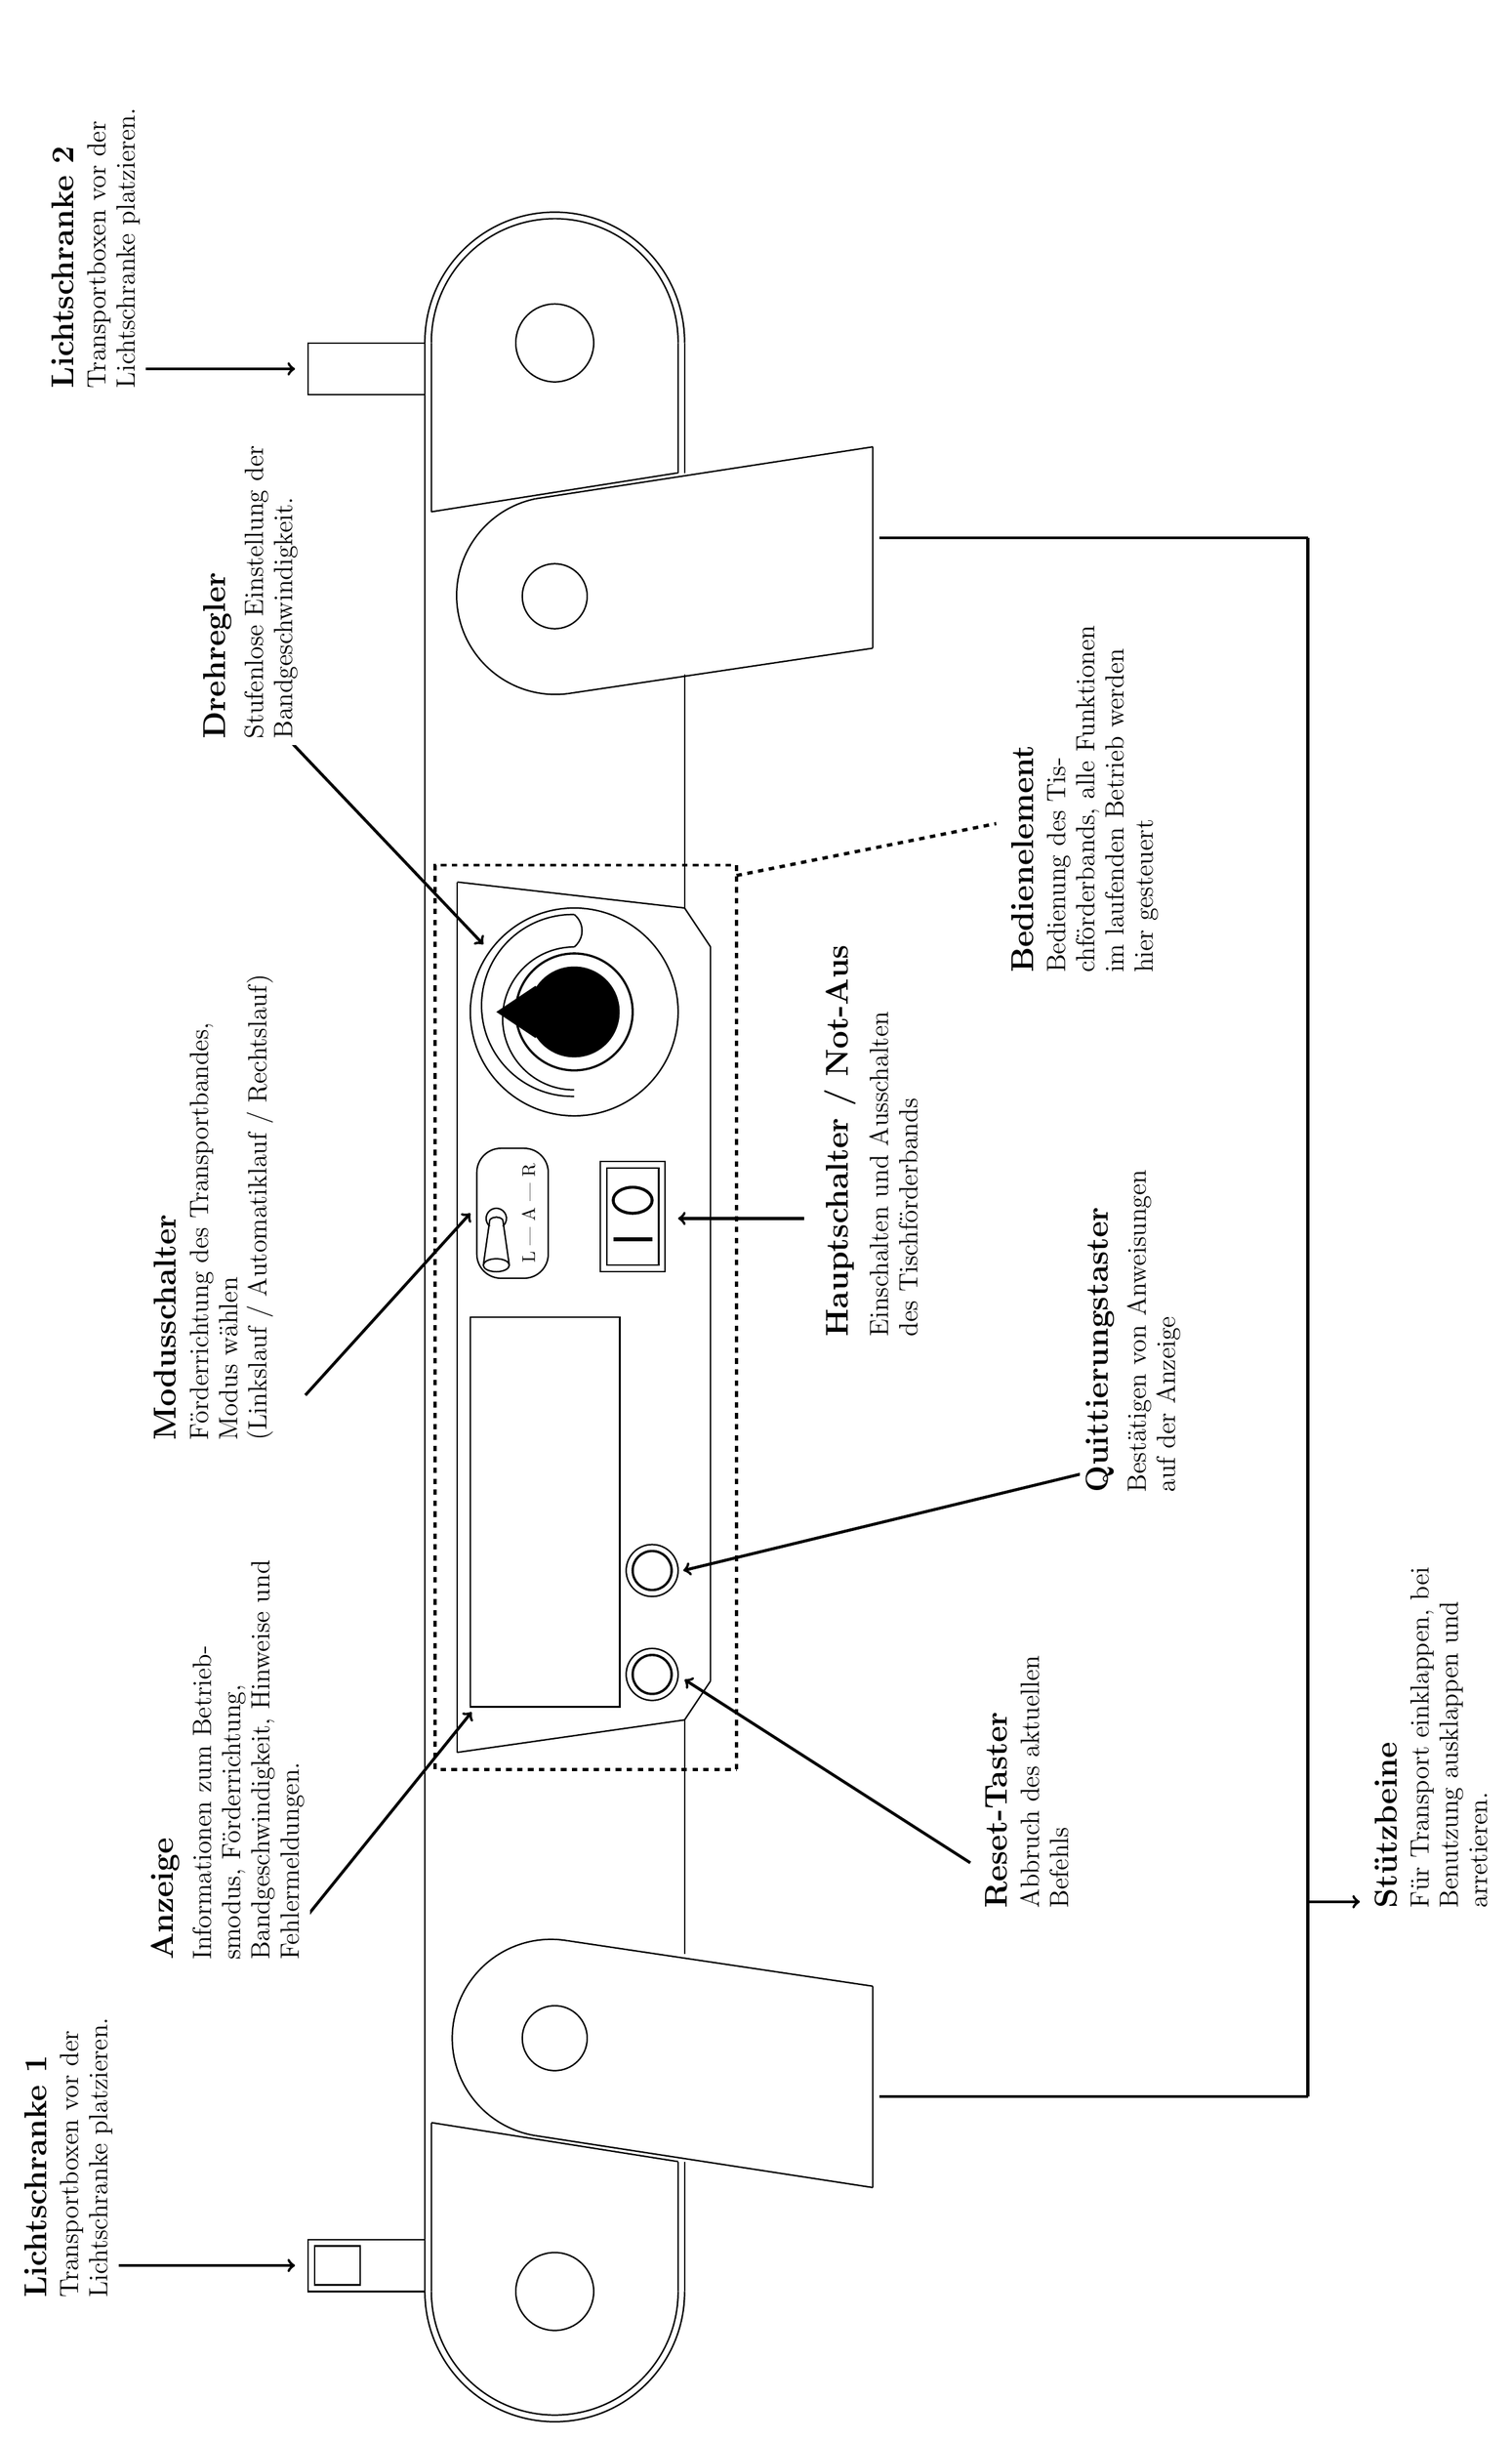
\begin{tikzpicture}[line width=0.8pt]
		
		
		
		\draw (20,-15.25) -- (20,22.25);
		\draw (25,22.25) -- (25,19.75);
		\draw (20,22.25) arc[start angle=-179.61, end angle=-360.39, radius=2.5001];
		\draw (25,-15.25) arc[start angle=0.15, end angle=-180.15, radius=2.5000];
		\draw (20.125,22.25) arc[start angle=-179.61, end angle=-360.39, radius=2.3751];
		\draw (24.875,22.25) -- (24.875,19.75);
		\draw (24.875,19.75) -- (20.125,19);
		\draw (20.125,19) -- (20.125,22.25);
		
		\draw (22.125,19.25) -- (28.625,20.25);
		\draw (28.625,20.25) -- (28.625,16.375);
		\draw (28.625,16.375) -- (22.75,15.5);
		\draw (22.75,15.5) arc[start angle=-82.86, end angle=-258.22, radius=1.9024];
		
		\draw (25,-15.25) -- (25,-12.75);
		\draw (24.875,-15.25) arc[start angle=0.08, end angle=-180.08, radius=2.3750];
		\draw (20.125,-15.25) -- (20.125,-12);
		\draw (24.875,-15.25) -- (24.875,-12.75);
		\draw (24.875,-12.75) -- (20.125,-12);
		
		\draw (22.125,-12.25) -- (28.625,-13.25);
		\draw (28.625,-13.25) -- (28.625,-9.375);
		\draw (28.625,-9.375) -- (22.75,-8.5);
		\draw (22.125,-12.25) arc[start angle=-99.16, end angle=-279.77, radius=1.9009];
		
		\draw (25,15.875) -- (25,11.375);				
		\draw (25,-4.25) -- (25,-8.75);
	% Lager Rollen	
		\draw (22.5,22.25) circle (0.75cm);
		\draw (22.5,-15.25) circle (0.75cm);
	% Drehpunkt klappbare Stützbeine
		\draw (22.5,17.375) circle (0.625cm);
		\draw (22.5,-10.375) circle (0.625cm);
	% Rahmen Bedienerpult	
		\draw (25,11.375) -- (20.625,11.875);
		\draw (20.625,11.875) -- (20.625,-4.875);
		\draw (20.625,-4.875) -- (25,-4.25);
		\draw (25,11.375) -- (25.5,10.625);
		\draw (25.5,10.625) -- (25.5,-3.5);
		\draw (25.5,-3.5) -- (25,-4.25);
	% Anzeige	
		\draw[line width=1pt] (20.875,3.5) rectangle (23.75,-4);
	% Lichtschranke 1	
		\draw (20,-15.25) rectangle (17.75,-14.25);
		\draw (17.875,-14.375) rectangle (18.75,-15.125);
	% Lichtschranke 2	
		\draw (20,22.25) rectangle (17.75,21.25);
		%\draw (17.875,22.125) rectangle (18.75,21.375);
		
	
	% Hauptschalter	
		\draw (23.375,4.375) rectangle (24.625,6.5);
		\draw (23.5,4.5) rectangle (24.5,6.375);
		\draw[line width=2pt] (24.375,5) -- (23.625,5);
		\draw[line width=1.6pt] (24,5.75) ellipse (0.375cm and 0.25cm);
		
	% Reset-Taster	
		\draw[line width=1.3pt] (24.375,-3.375) circle (0.375cm);
		\draw (24.375,-3.375) circle (0.5cm);
		
		\draw[line width=1.2pt] (22.875,9.375) circle (1.125cm);
		\draw (22.875,9.375) circle (2cm);
		
		\draw (22.875,7.875) arc[start angle=-89.84, end angle=-270.16, radius=1.3750];
		\draw (22.875,7.75) arc[start angle=-88.90, end angle=-271.10, radius=1.7503];
		\draw (22.875,11.25) arc[start angle=51.34, end angle=-51.34, radius=0.4002];
		
		\fill (22.875,9.375) circle (0.875cm);
		\fill (21.375,9.375) -- (22.125,8.875) -- (22.875,9.375) -- (22.125,9.875) -- cycle;
		
		\draw[rounded corners=13.2] (21,6.75) rectangle (22.375,4.25);
		\draw (21.25,5.375) -- (21.125,4.5);
		\draw (21.5,5.375) -- (21.625,4.5);
		\draw (21.375,4.5) ellipse (0.25cm and 0.125cm);
		\draw (21.25,5.375) arc[start angle=135, end angle=45, radius=0.1768];
		\draw (21.25,5.25) arc[start angle=-129.73, end angle=-410.27, radius=0.1956];
		
	% Beschriftungen (ohne lokale Fontdefinition)
		\node[rotate=90, fill=white] at (22,5.5) {L | A | R};
	

	
	% Reset-Taster	
		\draw[line width=1.6pt, ->] (30.5,-7) -- (25,-3.475);
		
		\node[
		rotate=90,
		anchor=west,
		fill=white,
		font=\fontsize{16pt}{18pt}\selectfont
		] (resettaster) at (31,-8)
		{\textbf{Reset-Taster}};
		
		\node[
		rotate=90,
		anchor=north west,
		text width=6cm,
		align=left,
		fill=white,
		font=\fontsize{14pt}{16pt}\selectfont
		] at (resettaster.south west)
		{Abbruch des aktuellen \\ Befehls};
	
	% Quittierungstaster
		\draw[line width=1.3pt] (24.375,-1.375) circle (0.375cm);
		\draw (24.375,-1.375) circle (0.5cm);
		\draw[line width=1.6pt, ->] (32.7,0.5) -- (24.975,-1.375);
		
		\node[
		rotate=90,
		anchor=west,
		fill=white,
		font=\fontsize{16pt}{18pt}\selectfont
		] (quittierung) at (33,0)
		{\textbf{Quittierungstaster}};
		
		\node[
		rotate=90,
		anchor=north west,
		text width=7cm,
		align=left,
		fill=white,
		font=\fontsize{14pt}{16pt}\selectfont
		] at (quittierung.south west)
		{Bestätigen von Anweisungen \\ auf der Anzeige};
	
	% Hauptschalter / Not-Aus
		\draw[line width=1.6pt, ->] (27.3,5.4) -- (24.875,5.4);
		
		\node[
		rotate=90,
		anchor=west,
		fill=white,
		font=\fontsize{16pt}{18pt}\selectfont
		] (hauptschalter) at (28,3)
		{\textbf{Hauptschalter / Not-Aus}};
		
		\node[
		rotate=90,
		anchor=north west,
		text width=7cm,
		align=left,
		fill=white,
		font=\fontsize{14pt}{16pt}\selectfont
		] at (hauptschalter.south west)
		{Einschalten und Ausschalten des Tischförderbands};
		
	% Stützbeine
		\draw[line width=1.6pt](28.75,18.5) -- (37,18.5);
		\draw[line width=1.6pt](37,18.5) -- (37,-11.5);
		\draw[line width=1.6pt] (37,-11.5) -- (28.75,-11.5);
		\draw[line width=1.6pt, ->] (37,-7.75) -- (38,-7.75);
		
		\node[
		rotate=90,
		anchor=west,
		fill=white,
		font=\fontsize{16pt}{18pt}\selectfont
		] (stuetzbeine) at (38.5,-8)
		{\textbf{Stützbeine}};
		
		\node[
		rotate=90,
		anchor=north west,
		text width=8cm,
		align=left,
		fill=white,
		font=\fontsize{14pt}{16pt}\selectfont
		] at (stuetzbeine.south west)
		{Für Transport einklappen, bei \\ Benutzung ausklappen und \\  arretieren.};
	
	% Lichtschranke 1
		\draw[line width=1.6pt, ->] (13.25,-14.75) -- (17.5,-14.75);
		
		\node[
		rotate=90,
		anchor=west,
		fill=white,
		font=\fontsize{16pt}{18pt}\selectfont
		] (licht1) at (12.5,-15.5)
		{\textbf{Lichtschranke 1}};
		
		\node[
		rotate=90,
		anchor=north west,
		text width=7cm,
		align=left,
		fill=white,
		font=\fontsize{14pt}{16pt}\selectfont
		] at (licht1.south west)
		{Transportboxen vor der \\ Lichtschranke platzieren.};
	
	% Lichtschranke 2
		\draw[line width=1.6pt, ->] (14.25,21.75) -- (17.5,21.75);
		
		\node[
		rotate=90,
		anchor=west,
		fill=white,
		font=\fontsize{16pt}{18pt}\selectfont
		] (licht2) at (13.025,21.25)
		{\textbf{Lichtschranke 2}};
		
		\node[
		rotate=90,
		anchor=north west,
		text width=7cm,
		align=left,
		fill=white,
		font=\fontsize{14pt}{16pt}\selectfont
		] at (licht2.south west)
		{Transportboxen vor der \\ Lichtschranke platzieren.};
	
	% Anzeige 
		\draw[line width=1.6pt, ->] (17.35,-8.5) -- (20.9,-4.1);
		
		\node[
		rotate=90,
		anchor=west,
		fill=white,
		font=\fontsize{16pt}{18pt}\selectfont
		] (anzeige) at (15,-9)
		{\textbf{Anzeige}};
		
		\node[
		rotate=90,
		anchor=north west,
		text width=8cm,
		align=left,
		fill=white,
		font=\fontsize{14pt}{16pt}\selectfont
		] at (anzeige.south west)
		{Informationen zum Betriebsmodus, Förderrichtung, Bandgeschwindigkeit, Hinweise und Fehlermeldungen.};
			
	% Drehregler
		\draw[line width=1.6pt, ->] (17.25,14.75) -- (21.125,10.675);
		
		\node[
		rotate=90,
		anchor=west,
		fill=white,
		font=\fontsize{16pt}{18pt}\selectfont
		] (drehregler) at (16,14.5)
		{\textbf{Drehregler}};
		
		\node[
		rotate=90,
		anchor=north west,
		text width=6cm,
		align=left,
		fill=white,
		font=\fontsize{14pt}{16pt}\selectfont
		] at (drehregler.south west)
		{Stufenlose Einstellung der \\ Bandgeschwindigkeit.};

	% Modusschalter	
		\draw[line width=1.6pt, ->] (17.7,2) -- (20.875,5.5);
		
		\node[
		rotate=90,
		anchor=west,
		fill=white,
		font=\fontsize{16pt}{18pt}\selectfont
		] (modusschalter) at (15,1)
		{\textbf{Modusschalter}};
		
		\node[
		rotate=90,
		anchor=north west,
		text width=9cm,
		align=left,
		fill=white,
		font=\fontsize{14pt}{16pt}\selectfont
		] at (modusschalter.south west)
		{Förderrichtung des Transportbandes, \\ Modus wählen\\
			(Linkslauf / Automatiklauf / Rechtslauf)};
			
	% Bedienerpult 
		\draw[dashed, line width=1.8pt](26,-5.2) rectangle (20.2,12.2);
		\draw [dashed, line width=1.8pt] (26,12) -- (31,13);
		
		\node[
		rotate=90,
		anchor=west,
		fill=white,
		font=\fontsize{16pt}{18pt}\selectfont
		] (bedienelement) at (31.5,10)
		{\textbf{Bedienelement}};
		
		\node[
		rotate=90,
		anchor=north west,
		text width=7cm,
		align=left,
		fill=white,
		font=\fontsize{14pt}{16pt}\selectfont
		] at (bedienelement.south west)
		{Bedienung des Tischförderbands, alle Funktionen im laufenden Betrieb werden hier gesteuert};
			
	\end{tikzpicture}
}
	\caption{Übersicht der Bedienerelemente, Vorderansicht}
	\end{center}
\end{figure}

% Skizze 2

\begin{figure}[!ht]
	
	\begin{center}
		\resizebox{0.7\textwidth}{!}{%
			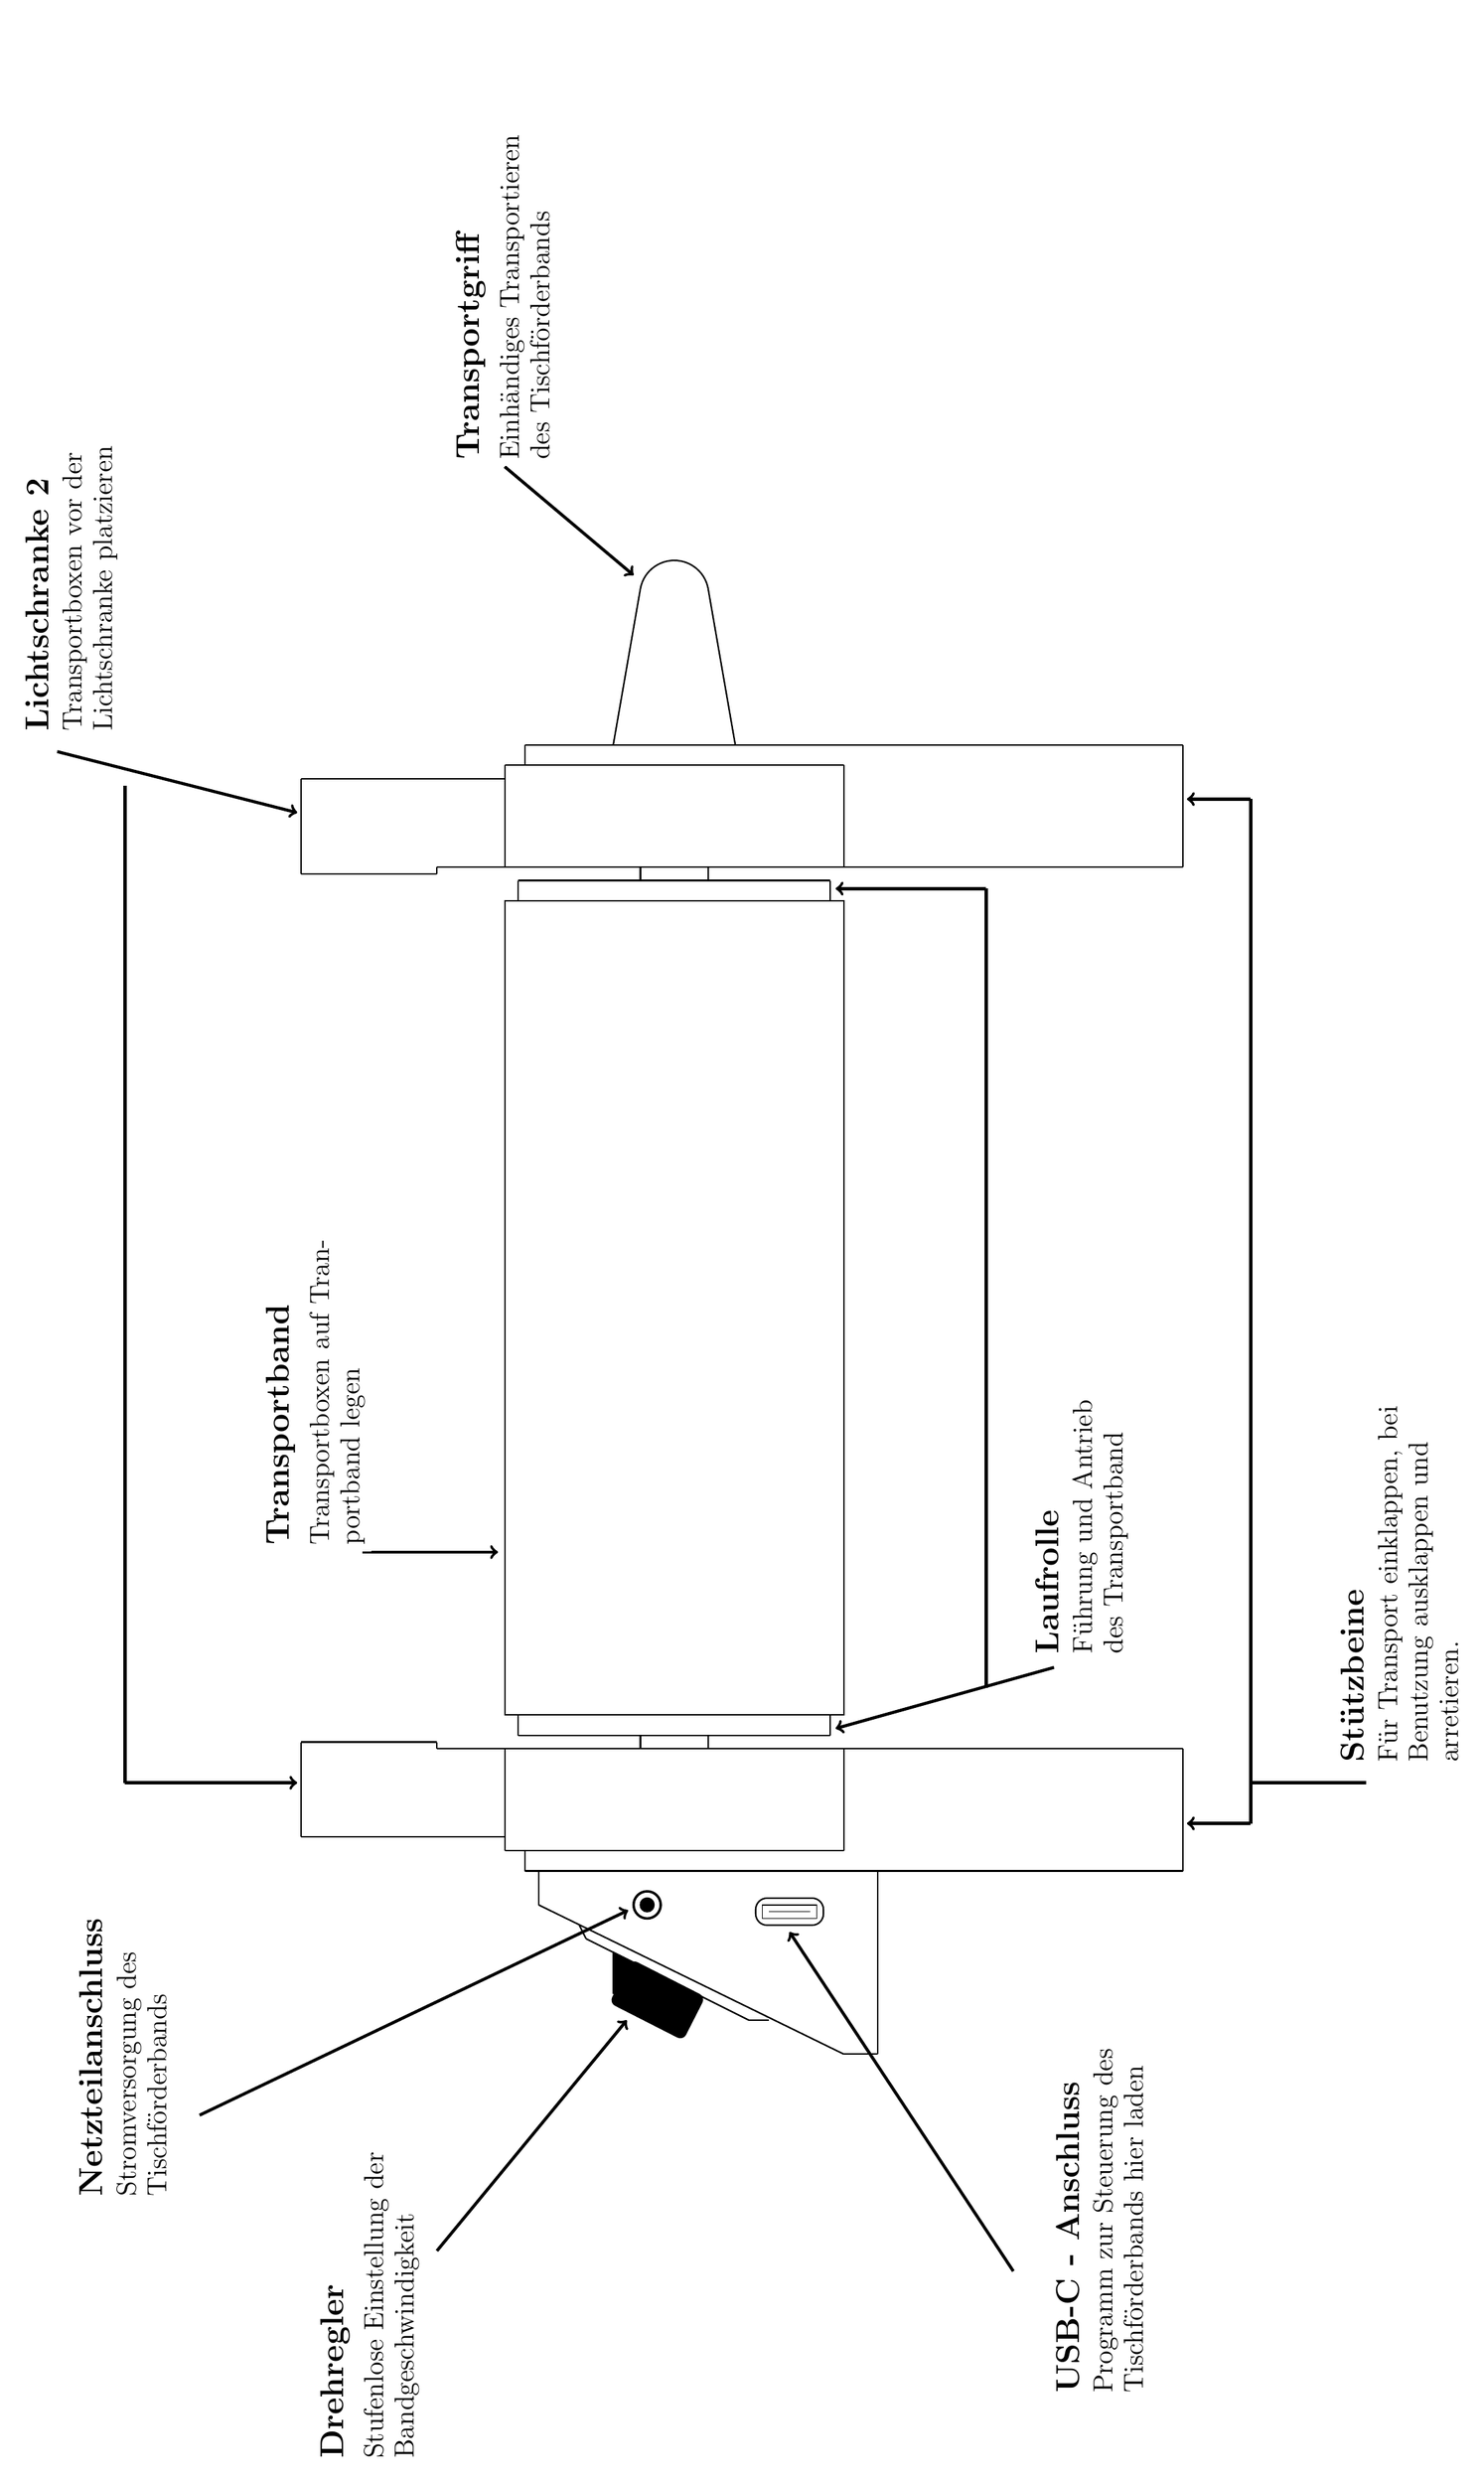
\begin{tikzpicture}[line width=0.8pt, rotate=90,
								transform shape]
				
				\draw  (5,7.375) rectangle (20,1.125);
				\draw  (5,7.125) -- (4.625,7.125);
				\draw  (4.625,1.375) -- (5,1.375);
				\draw  (20,7.125) -- (20.375,7.125);
				\draw  (20,1.375) -- (20.375,1.375);
				\draw  (20.625,7.375) -- (22.5,7.375);
				\draw  (22.5,7.375) -- (22.5,1.125);
				\draw  (22.5,1.125) -- (20.625,1.125);
				\draw  (4.375,7.375) -- (2.5,7.375);
				\draw  (2.5,7.375) -- (2.5,1.125);
				\draw  (2.5,1.125) -- (4.375,1.125);
				\draw  (20.375,7.125) -- (20.375,4.875);
				\draw  (20.375,1.375) -- (20.375,3.625);
				\draw  (20.375,4.875) rectangle (20.625,3.625);
				\draw  (20.625,7.375) -- (20.625,4.875);
				\draw  (20.625,3.625) -- (20.625,-5.125);
				\draw  (4.625,7.125) -- (4.625,4.875);
				\draw  (4.625,1.375) -- (4.625,3.625);
				\draw  (4.625,4.875) rectangle (4.375,3.625);
				\draw  (4.375,7.375) -- (4.375,4.75);
				\draw  (4.375,3.625) -- (4.375,-5.125);
				\draw  (2.125,6.75) -- (1.5,6.75);
				\draw  (1.5,6.75) -- (-1.25,1.125);
				\draw  (-1.25,0.5) -- (2.125,0.5);
				\draw  (20.625,-5.125) -- (22.875,-5.125);
				\draw  (22.875,-5.125) -- (22.875,7);
				\draw  (22.5,7) -- (22.875,7);
				\draw  (2.125,-5.125) -- (2.125,7);
				\draw  (2.125,-5.125) -- (4.375,-5.125);
				\draw  (2.125,7) -- (2.5,7);
				\draw  (22.875,5.375) -- (25.75,4.875);
				\draw  (25.75,4.875) arc[start angle=79.84, end angle=-79.84, radius=0.6350];
				\draw  (25.75,3.625) -- (22.875,3.125);
				\draw  (20.625,7.375) -- (20.625,8.625);
				\draw  (20.625,8.625) -- (20.5,8.625);
				\draw  (20.5,8.625) -- (20.5,11.125);
				\draw  (20.5,11.125) -- (22.25,11.125);
				\draw  (22.25,11.125) -- (22.25,7.375);
				\draw  (-1.25,1.125) -- (-1.25,0.5);
				\draw  (-0.625,2.5) -- (-0.625,2.875);
				\draw  (-0.625,2.875) -- (0.875,5.875);
				\draw  (0.875,5.875) -- (1.125,6);
			
			% Drehregler
				\draw[fill=black] (0.125,4.375) -- (-0.625,4.375) -- (-0.125,5.375) -- (0.625,5.375) -- cycle;
				\draw[fill=black, rounded corners=3pt, rotate around={-117:(-0.25,4.5625)}] 
				(-1,5) rectangle (0.5,4.125);
			
			% Netzteilanschluss			
				\draw[line width=1.3pt] (1.5,4.75) circle (0.25cm);
				\draw[fill=black] (1.5,4.75) circle (0.125cm);
			
			% USB-C Anschluss		
				\draw[line width=0.8pt, rounded corners=6pt] (1.125,2.75) rectangle (1.625,1.5);
				\draw[line width=0.6pt] (1.25,2.625) rectangle (1.5,1.625);
				\draw[line width=0.6pt] (1.375,2.5) -- (1.375,1.75);
				
			% Lichtschranke Reflektor
				\draw (2.75,11.125) -- (4.5,11.125);
				\draw (2.75,11.125) -- (2.75,7.375);
				\draw (4.5,8.625) -- (4.5,11.125);
				\draw (4.5,8.625) -- (4.375,8.625);
				\draw (4.375,7.375) -- (4.375,8.625);	

	% ---------------- gestrichelte Linien ------------	
		
		% Transportband
			\draw[line width=1.6pt, <-] (8,7.5) -- (8,10);
			
		% Laufrolle	
			\draw[line width=1.6pt, <-] (4.75,1.275) -- (5.875,-2.75);                 
			\draw[line width=1.6pt, <-] (20.225,1.275) -- (20.225,-1.5);               
			\draw[line width=1.6pt] (20.225,-1.5) -- (5.5,-1.5);                  
		
		% USB-C - Anschluss
			\draw[line width=1.6pt, <-] (1,2.125) -- (-5.25,-2);                    
		
		% Netzkabel-Anschluss
			\draw[line width=1.6pt, <-] (1.4,5.1) -- (-2.375,13);                
		
		% Drehregler
			\draw[line width=1.6pt, <-] (-0.625,5.125) -- (-4.875,8.625);              
		
		% Stützbeine
			\draw[line width=1.6pt, <-] (3,-5.2) -- (3,-6.375);                      
			\draw[line width=1.6pt] (3,-6.375) -- (21.875,-6.375);                 
			\draw[line width=1.6pt, ->] (21.875,-6.375) -- (21.875,-5.2);            
			\draw[line width=1.6pt] (3.75,-6.375) -- (3.75,-8.5);                    
		 % Lichtschranke 2
			\draw[line width=1.6pt, <-] (21.625,11.2) -- (22.75,15.625);            
			\draw[line width=1.6pt] (3.75,14.375) -- (22.125,14.375);  
			\draw[line width=1.6pt, <-] (3.75,11.2) -- (3.75,14.375);
			
		 % Transportgriff
			\draw[line width=1.6pt, <-] (26,5) -- (28,7.375);                   
					
	% ------------------ TEXTFELDER ------------------
		
		% Transportband
			\node[
			anchor=west,
			fill=white,
			font=\fontsize{16pt}{18pt}\selectfont
			] (transportband) at (8,11.5)
			{\textbf{Transportband}};
			
			\node[
			anchor=north west,
			text width=6.5cm,
			align=left,
			fill=white,
			font=\fontsize{14pt}{16pt}\selectfont
			] at (transportband.south west)
			{Transportboxen auf Tranportband legen};
		
		% Laufrolle
			\node[
			anchor=west,
			fill=white,
			font=\fontsize{16pt}{18pt}\selectfont
			] (laufrolle) at (6,-2.625)
			{\textbf{Laufrolle}};
			
			\node[
			anchor=north west,
			text width=6.5cm,
			align=left,
			fill=white,
			font=\fontsize{14pt}{16pt}\selectfont
			] at (laufrolle.south west)
			{Führung und Antrieb \\ des Transportband};
			
			
			
		% USB-C Anschluss
			\node[
			anchor=west,
			fill=white,
			font=\fontsize{16pt}{18pt}\selectfont
			] (usbc) at (-7.625,-3)
			{\textbf{USB-C - Anschluss}};
			
			\node[
			anchor=north west,
			text width=7cm,
			align=left,
			fill=white,
			font=\fontsize{14pt}{16pt}\selectfont
			] at (usbc.south west)
			{Programm zur Steuerung des Tischförderbands hier laden};
			
			
		% Netzteilanschluss
			\node[
			anchor=west,
			fill=white,
			font=\fontsize{16pt}{18pt}\selectfont
			] (netzteil) at (-4,15)
			{\textbf{Netzteilanschluss}};
			
			\node[
			anchor=north west,
			text width=7cm,
			align=left,
			fill=white,
			font=\fontsize{14pt}{16pt}\selectfont
			] at (netzteil.south west)
			{Stromversorgung des \\ Tischförderbands};
			
			
			
		% Drehregler
			\node[
			anchor=west,
			fill=white,
			rounded corners=2pt,
			font=\fontsize{16pt}{18pt}\selectfont
			] (drehregler2) at (-8.83,10.5)
			{\textbf{Drehregler}};
			
			\node[
			anchor=north west,
			text width=7cm,
			align=left,
			fill=white,
			font=\fontsize{14pt}{16pt}\selectfont
			] at (drehregler2.south west)
			{Stufenlose Einstellung der \\ Bandgeschwindigkeit};
			
			
			
		% Stützbeine
			\node[
			anchor=west,
			fill=white,
			font=\fontsize{16pt}{18pt}\selectfont
			] (stuetzbeine2) at (4,-8.25)
			{\textbf{Stützbeine}};
			
			\node[
			anchor=north west,
			text width=8cm,
			align=left,
			fill=white,
			font=\fontsize{14pt}{16pt}\selectfont
			] at (stuetzbeine2.south west)
			{Für Transport einklappen, bei \\ Benutzung ausklappen und \\  arretieren.};
			
			
			
		% Lichtschranke 2
			\node[
			anchor=west,
			fill=white,
			font=\fontsize{16pt}{18pt}\selectfont
			] (lichtschranke2b) at (23,16)
			{\textbf{Lichtschranke 2}};
			
			\node[
			anchor=north west,
			text width=7cm,
			align=left,
			fill=white,
			font=\fontsize{14pt}{16pt}\selectfont
			] at (lichtschranke2b.south west)
			{Transportboxen vor der Lichtschranke platzieren};
			
			
			
		% Transportgriff
			\node[
			anchor=west,
			fill=white,
			font=\fontsize{16pt}{18pt}\selectfont
			] (transportgriff) at (28,8)
			{\textbf{Transportgriff}};
			
			\node[
			anchor=north west,
			text width=8cm,
			align=left,
			fill=white,
			font=\fontsize{14pt}{16pt}\selectfont
			] at (transportgriff.south west)
			{Einhändiges Transportieren \\ des Tischförderbands};
			
		\end{tikzpicture}	
			} % resizebox
		\end{center}
		
		\caption{Übersicht der Bedienerelemente, Seitenansicht}
		
	\end{figure}